\subsection{Schritt 1 - Formular in Grundstruktur erstellen}

Im ersten Schritt soll die Formular-Anwendung in ihrer Grundstruktur entwickelt werden.  Das beinhaltet alle drei Oberflächen, welche in den darauf folgenden Schritten lediglich erweitert werden.  Das Formular erhält noch keine  Validierung. Somit sind alle Eingaben oder nicht kompatible Selektionen erlaubt.Die erste Ansicht, welche der Benutzer sieht, soll die Übersicht der bereits eingetragenen Maßnahmen sein \Abb{\ref{fig:Schritt1Uebersicht}}.

% TODO: rausgekürzt, doch wieder rein nehmen?
%Dort ist auch zu sehen, dass die Anwendung ohne Anpassungen zunächst einmal im sogenannten Material Design\footnoteI{Material Design umfasst eine Reihe von Prinzipien zur Auszeichnung von Benutzeroberflächen. Das ist Design-System wurde von Google Inc. entwickelt.  Der Name leitet sich daher ab, dass Objekte mit der Nachahmung physikalischer Eigenschaften - wie etwa dem Werfen eines Schattens - den Eindruck von tatsächlichen Materialien erwecken. \footnote{\cite{MaterialDesignIntroduction}}} gestylt ist.
\begin{figure}[H]
  \centering
  \includegraphics[width=1.0\textwidth]{Inhalt/Hauptteil/Implementierung/Schritt-1/Übersicht.png}
  \caption[Schritt 1 Übersicht]{Der Übersicht-Bildschirm zeigt in  Schritt 1 zunächst nur die Maßnahmen mit ihrem Titel und Bearbeitungsdatum in den Kategorien \enquote{Abgeschlossen} und \enquote{In Bearbeitung}. Quelle: Eigene Abbildung}
  \label{fig:Schritt1Uebersicht}
\end{figure}
Die Auflistung der Maßnahmen erfolgt in den Kategorien \enquote{In Bearbeitung} und \enquote{Abgeschlossen}. Innerhalb dieser Rubriken werden die Maßnahmen in einer Tabelle angezeigt. Mit einem Klick auf den Button unten rechts im Bild wird der Benutzer auf die zweite Ansicht weitergeleitet: die Eingabemaske \Abb{\ref{fig:Schritt1Eingabemaske}}.
\begin{figure}[H]
  \centering
  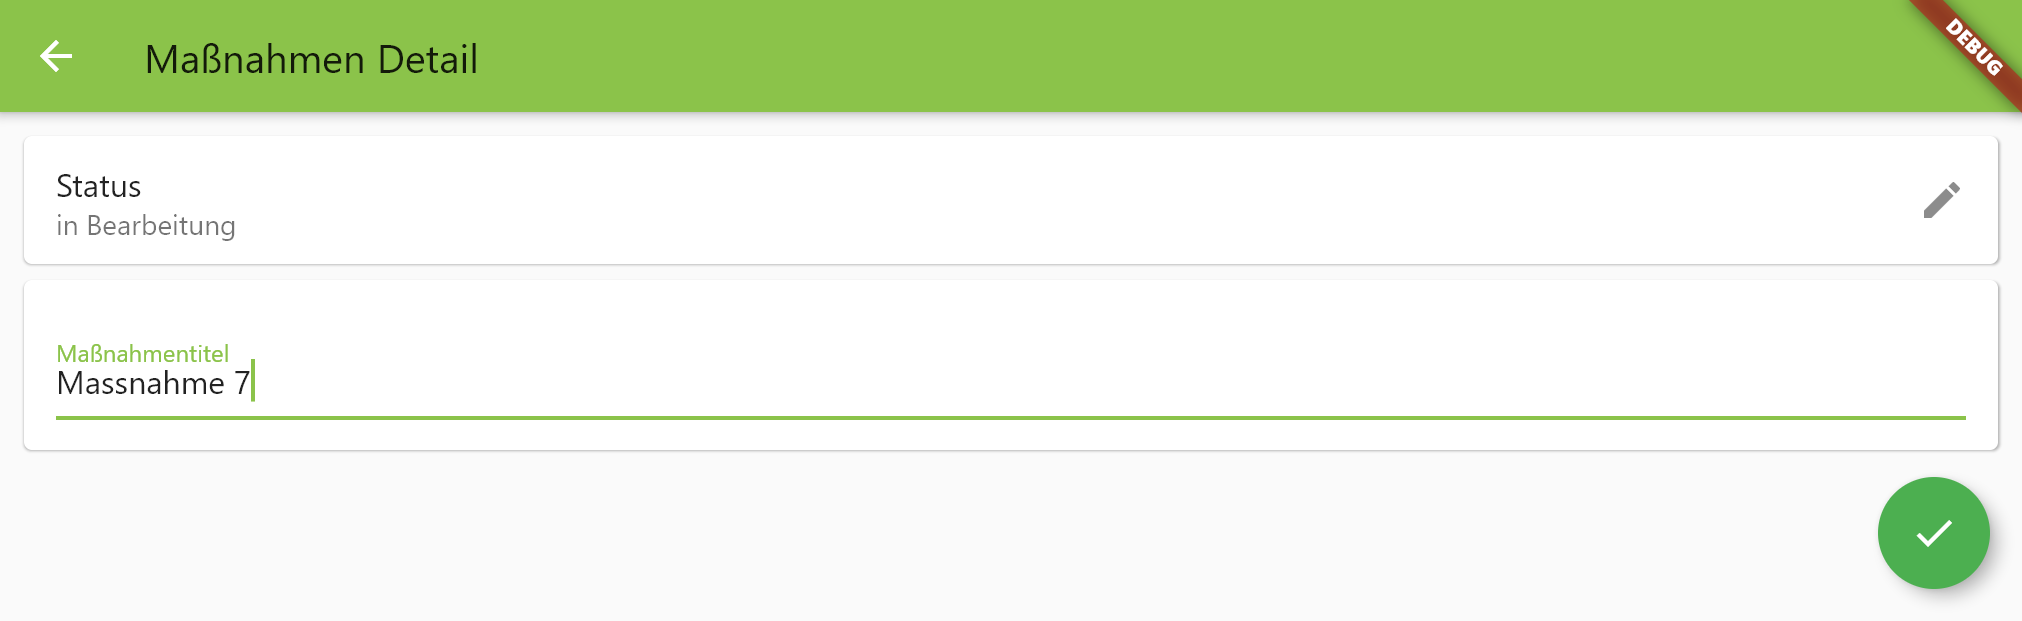
\includegraphics[width=1.0\textwidth]{Inhalt/Hauptteil/Implementierung/Schritt-1/Eingabemaske.png}
  \caption[Schritt 1 Eingabemaske]{Die Eingabemaske zeigt im Schritt 1 eine Karte zum Selektieren des Status und ein Eingabefeld für den Titel. Quelle: Eigene Abbildung}
  \label{fig:Schritt1Eingabemaske}
\end{figure}
Sie ermöglicht die Eingabe des Maßnahmen-Titels über ein simples Eingabefeld. Darüber hinaus ist die Selektions-Karte für den Status zu sehen. Mit einem Klick auf diese Karte öffnet sich der Selektions-Bildschirm. Er ermöglicht die Auswahl der Auswahloptionen, in diesem Fall die Optionen \enquote{in Bearbeitung} und \enquote{abgeschlossen}
\Abb{\ref{fig:Schritt1SelektionsBildschirmStatus}}.

\begin{figure}[H]
  \centering
  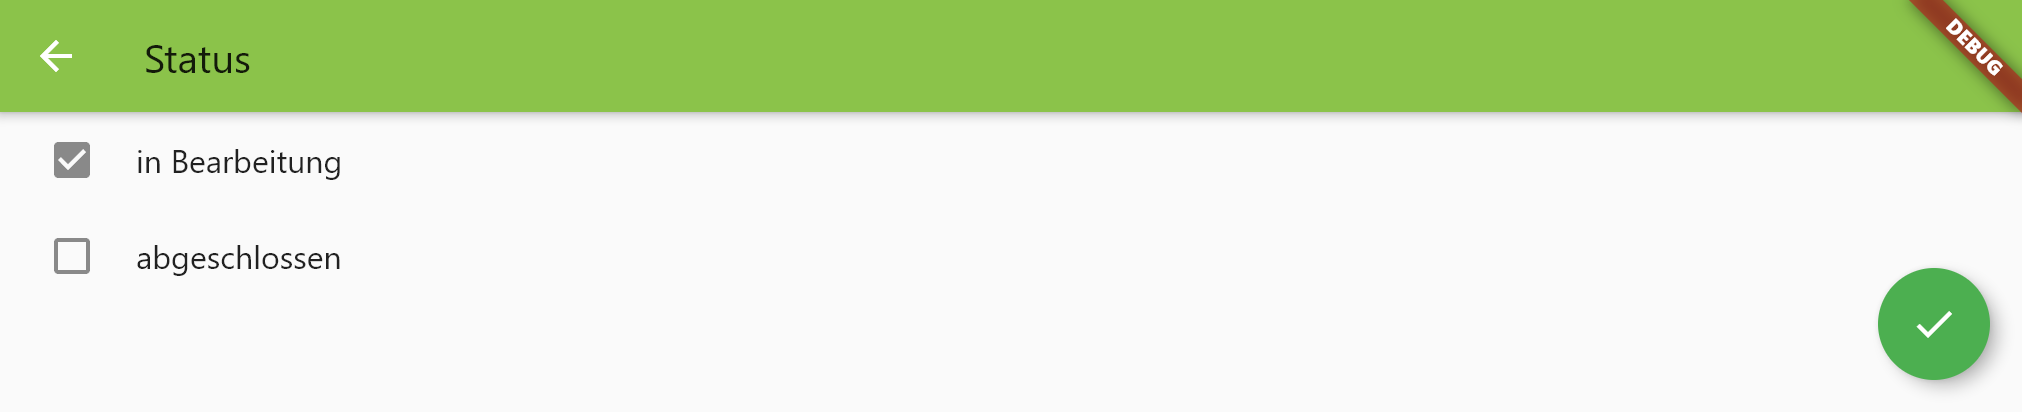
\includegraphics[width=1.0\textwidth]{Inhalt/Hauptteil/Implementierung/Schritt-1/Status Auswahl.png}
  \caption[Schritt 1 Selektions-Bildschirm für Status]{Der Selektions-Bildschirm für das Feld Status erlaubt die Auswahl der Optionen \enquote{in Bearbeitung} und \enquote{abgeschlossen}. Quelle: Eigene Abbildung}
  \label{fig:Schritt1SelektionsBildschirmStatus}
\end{figure}

% TODO: rausgekürzt, doch wieder rein nehmen?
%\footnoteI{Ein floating action button (FAB) ist im Material Design ein Button, der über der Benutzeroberfläche schwebt und daher dem Benutzer leicht ins Auge fällt. Aus diesem Grund wird er für primäre Aktionen genutzt - in diesem Fall dem Erstellen einer neuen Maßnahme. \footnote{\cite{MaterialDesignFloatingActionButton}}} ist in der unteren rechten Ecke der Ansicht zu finden. Mit einem Klick darauf wird der Benutzer auf die zweite Ansicht weitergeleitet: die Eingabemaske. 

\subsubsection{Auswahloptionen hinzufügen}

Dart verfügt – anders als beispielsweise Java\footcite[Vgl.][S. 321]{TheJavaLanguageSpecificationJavaSE16Edition} – nicht über Aufzählungstypen mit zusätzlichen Eigenschaften. Das Schlüsselwort \mintinline{dart}{enum} in Dart erlaubt lediglich die Auflistung konstanter Symbole\footcite[Vgl.][S. 74f.]{DartProgrammingLanguageSpecification5thedition}. Für die Auswahl Optionen ist es jedoch notwendig, dass es zwei Eigenschaften gibt:
\begin{itemize}
  \parsep 0pt
  \topsep 0pt
  \itemsep 0pt

  \item die Abkürzung, die in der resultierendem Datei gespeichert werden soll
  \item und der Beschreibungstext, welcher in der Oberfläche angezeigt wird.
\end{itemize}
Das hat den Hintergrund, dass die Abkürzungen weniger Speicherplatz einnehmen und die Beschreibung sich in Zukunft auch ändern darf. Würde anstatt der Abkürzung die Beschreibung als Schlüssel verwendet werden, so würde eine Datei, die mit einer älteren Version des Formulars erstellt wurde, nicht mehr von neueren Versionen der Applikationeingelesen werden können. Der alte Beschreibungstext würde nicht mehr mit dem Text übereinstimmen, der als Schlüssel in der Anwendung verwendet wird.


Die beiden Zustände \enquote{in Bearbeitung} und \enquote{abgeschlossen} werden daher in Listing \ref{Schritt1KlasseLetzterStatus} als statische Klassenvariablen deklariert \Z{6-7}. Die beiden Konstruktor-Aufrufe übergeben dabei als erstes Argument die Abkürzung und als zweites Argument die Beschreibung. Der Konstruktor selbst \Z{9-10} deklariert die beiden Parameter als positionale Parameter.

\begin{alexlisting}{Schritt 1}{Die Klasse LetzterStatus}
  {Quellcode/Schritt-1/conditional_form/lib/choices/choices.dart}
  {firstline=5, lastline=11}
  \label{lst:Schritt1KlasseLetzterStatus}
\end{alexlisting}

\paragraph{Positionale Parameter}

Im Vergleich zu den benannten Parametern ist bei den positionalen Parametern nur ihre Reihenfolge in der Parameterliste ausschlaggebend. Das Argument für die \IC{abbreviation} steht dabei also immer an erster Stelle und das Argument für \IC{description} immer an der zweiten \Z{6-7}. Positionale Parameter sind vorgeschrieben. Werden sie ausgelassen, so gibt es einen Compilerfehler. \DartSpec{74f.}

Die Klasse \IC{LetzterStatus} erbt von der Basisklasse \IC{Choice} \Z{5}. Der Konstruktor der Klasse \Z{9} übergibt beide Parameter als Argumente an den Konstruktor der Klasse \IC{Choice}. Genau wie in Java wird mithilfe des Schlüsselwortes \IC{super}\Z{10} der Konstruktor der Basisklasse aufgerufen. Doch anders als in Java erfolgt der Aufruf des super Konstruktors nicht in der ersten Zeile des Konstruktor-Körpers \JavaSpec{310}. Weil das Aufrufen des Konstruktors der Basisklasse zum statischen Teil der Objekt-Instanziierung gehört, muss der Aufruf von \IC{super} in der Initialisierungsliste erfolgen. Die Initialisierungsliste wird mit dem \IC{:} nach der Parameterliste eingeleitet \Z{10}\DartSpec{42}.

Die Basisklasse \IC{Choice} \Lst{\ref{lst:Schritt1KlasseChoice}} deklariert lediglich die beiden Felder \IC{description} und \IC{abbreviation} jeweils als \IC{String} \Z{4-5}. Beide sind mit \IC{final} gekennzeichnet, was sie zu unveränderlichen Instanzvariablen macht. Nach der Initialisierung, können sie keine anderen Werte annehmen. \DartSpec{S16} Die Initialisierung der beiden Variablen muss im statischen Kontext der Instanziierung erfolgen. Mit der abgekürzten Schreibweise \IC{this.abbreviation} und \IC{this} \IC{.description} im Konstruktor \Z{7} werden die Parameter den Feldern zugewiesen.

\begin{alexlisting}{Schritt 1}{Die Klasse Choice}
  {Quellcode/Schritt-1/conditional_form/lib/choices/base/choice.dart}
  {firstline=3, lastline=7}
  \label{lst:Schritt1KlasseChoice}
\end{alexlisting}

Dies erübrigt sowohl die Angabe des Parametertypes mittels \IC{(String abbreviation, String description)}, denn der Typ des Parameters kann bereits durch Angabe des Typs in der Instanzvariablen-Deklaration\Z{4-5} abgeleitet werden. Außerdem entfällt auch die Zuweisung, die man ansonstenin der Form \IC{this.abbreviation = abbreviation} und \IC{this.}\IC{description = description} in der Initialisierungsliste erreichen würde.\DartSpec{40f}
% Auch String description wird gespart


\begin{alexlisting}{Schritt 1}{Die Menge letzterStatusChoices}
  {Quellcode/Schritt-1/conditional_form/lib/choices/choices.dart}
  {firstline=13}
  \label{lst:Schritt1DieMengeLetzterStatusChoices}
\end{alexlisting}

Die Variable \IC{letzterStatusChoices} fasst die beiden statischen Klassenvariablen als eine Kollektion zusammen. Da es sich um eine solche Kollektion handelt, in der jedes Element nur ein einziges Mal vorkommen darf, ist hier von einer Menge zu sprechen. Auffällig hier ist, dass das Schlüsselwort new fehlt. In Dart ist das Schlüsselwort für die Konstruktion von Instanzen optional.  Die Klasse, die zur Konstruktion dieser Menge verwendet wird, ist die selbst erstellte Klasse choices. Über das Typargument LetzterStatus wird erreicht, das ausschließlich Variablen  dieses Typs in der Menge eingefügt werden dürfen. Wird stattdessen eine Variable eingefügt, die weder vom selben Typ, noch von einem Typ, der von letzter Status erbt, so gibt es einen Compilerfehler. Dies dient einzig und allein dem Zweck, dem  Fehler vorzubeugen, dass aus Versehen falsche Optionen in der Menge eingetragen werden. Über den Parameter name ist es möglich dieser Menge die Beschriftung “Status” hinzuzufügen.  Es handelt sich hier um einen  benamten Parameter.

Listing 4 zeigt die Klasse choices. Sie erbt von UnmodifiableSetView und erlaubt damit die Erstellung  einer eigenen Menge - auch Set genannt. Methoden, die man von einem Set erwartet,  lassen sich somit direkt auf  Instanzen der Klasse Choices aufrufen. Darunter unter anderem die contains Methode,  welche erlaubt, das Vorhandensein eines Objektes im Set zu überprüfen.
%   todo Referenz contains einfügen
%    todo Referenz UnmodifiableSetView
Instanzvariable name -  deklariert in Zeile 11 - wird im Konstruktor in Zeile 16 zugewiesen. Auffällig hierbei ist, dass der Parameter in geschweiften Klammern geschrieben steht und das Schlüsselwort required  vorangestellt ist. Das macht den Parameter zu einem vorgeschriebenen benannten Parameter.

\paragraph{Vorgeschriebene benamte Parameter}

Gewöhnlicher benannte Parameter sind optional. Wird ihnen das Schlüsselwort \IC{required} vorangestellt, so müssen sie gesetz werden, denn sonst gibt es einen Compilerfehler.  An dieser Stelle ist das \IC{required} Schlüsselwort sinnvoll, denn es handelt sich um den Datentyp String der nicht den  wert \IC{null} annehmender. Würde  der Parameter aber optional sein, so wäre es möglich, das programm zu kompilieren, auch wenn bei Aufrufen des Konstruktors kein Argument für den Parameter übergeben wurde. Doch in diesem Fall gäbe es keinen Initialwert für Name und somit müsste der  Instanzvariable null  zugewiesen werden. in der statischen Analyse wird daher sichergestellt, das Instanzvariablen durch benannte Parameter nur dann initialisiert werden dürfen, wenn dieser durch required  als vorgeschrieben gekennzeichnet sind und damit unter keinem Umstand ausgelassen werden können. Dürfte name den Wert Null annehmen, So würde es sich um den nullable Datentyp String  mit der Notation String? Handeln.

\paragraph{Typen ohne NULL-Zulässigkeit} Im Vergleich zu vielen anderen Programmiersprachen wie beispielsweise in Java wird in Dart zwischen gewöhnlichen Typen und nullable Typen unterschieden. In Sprachen wie Beispielsweise Java ist es nur bei atomaren Datentypen wie int und float vorgeschrieben einen Wert anzugeben. Null ist bei diesen primitiven Datentypen nicht als Wert erlaubt. Doch nicht atomare Datentypen erlauben immer die Angabe von Null als wert. Null drückt dabei immer das Nichtvorhandensein von Daten aus. Ab Dart 2.12   kann allen Datentypen standardmäßig keinen neuen Wert zugewiesen werden.  das hat den Vorteil, dass der Compiler sich darauf verlassen kann, das eine Variable niemals den Wert 0 haben kann. Das ist besonders dann nützlich, wenn auf  Einem Objekt eine Methode aufgerufen wird. Ist die Referenz das Objekt ist in Wahrheit 0 so gibt es erst zur Laufzeit einen Fehler, dass die Methode auf der Referenz \IC{null}nicht aufgerufen werden kann. Damit  ein Laufzeitfehler geworfen werden kann, muss vor jedem Aufruf einer Methode auf einer Referenz überprüft werden, ob die Referenzen nicht \IC{null} sind. Würde diese Überprüfung nicht stattfinden, so  könnte kein Laufzeitfehler geworfen werden und das Programm würde ohne Fehlermeldung abstürzen. Handelt es sich allerdings um eine Referenz, die niemals den Wert 0 annehmen kann, so kann der Compiler die Überprüfung auf 0 Wörter für diese Referenzen überspringen. Damit hört zusätzlich die Ausführungsgeschwindigkeit erhöht, da die  Überprüfung auf \IC{null}Zeit in Anspruch nimmt. Vor allem aber ist das forderheft für den Wickler, da der Compiler  Fehlermeldungen und Warnungen mitteilen kann, wenn  Operationen  mit Variablen mit potenziellen \IC{null}  Werten verwendet werden.

Neben Name wird mit  choiceByAbbreviation eine weitere Instanzvariable deklariert 12.
es handelt sich um den Datentyp map -  eine Kollektion die Daten mittels Schlüssel Wertepaaren ablegen kann.   als Schlüssel wird  die Abkürzung mit dem Datentyp String verwendet. Als wert ist der  generische typ Parameter t angegeben.  der typ Parameter ist in Zeile zehn deklariert und muss  mindestens von der Klasse Joyce erben. In choiceByAbbreviation werden also die Auswahlmöglichkeiten über  ihre Abkürzung abgelegt und können über dieselbe wieder referenziert werden.  Da es sich auch hier um eine unveränderliche Instanzvariable handelt, muss sie schon in der Initialisierungsliste initialisiert werden 17 bis 19. Dabei wird zunächst mit der öffnenden geschweiften Klammer 17 ein sogenanntes Map Literal begonnen, welches mit  schließenden geschweiften Klammer 19 endet.

\paragraph{Set und Map Literale}

Dart erlaubt es  setz und Maps als sogenannte literale zu deklarieren. es entfällt also die Instanziierung eines Sets oder einer Map über den Klassennamen und der darauffolgenden Zuweisung der einzelnen Werte. Stattdessen startet das literal mit einer öffnenden geschweiften Klammer und endet mit einer  schließenden geschweiften Klammer Punkt innerhalb der Klammern werden die Werte im Fall eines Sets  mit, getrennt nacheinander aufgeführt. Im Fall einer Map werden der Schlüssel und der Wert durch einen : voneinander getrennt und die Schlüsse Wertepaare wiederum durch, getrennt nacheinander aufgelistet.

Auffällig ist jedoch, dass In Zeile 18 dem Set lateral keine  einfache Auflistung von Werten übergeben wird. Stattdessen wird das mit dem sogenannte collection for eine wiederholung verwendet.

\paragraph{Collection for} Dart erlaubt es Schleifen innerhalb von Listen-, Set- und Map-Literalen zu verwenden. Dabei darf die Schleife jedoch keinen steifen Körper besitzen. Ledig der Schleifenkopf wird dazu in das literal selbstgeschrieben gefolgt von dem Wert, der bei jedem Schleifendurchlauf  dem literal hinzugefügt werden soll. Da wir kann der Wert von der Schleifen variable abgeleitet werden.  In Zeile 18 wird beispielsweise durch die  Menge aller Auswahloptionen choices iteriert und dabei in jedem Schleifendurchlauf  die Ausweise Option in die Variablen choice gespeichert. Während des Schleifendurchlauf wird dann ein Wertepaar gebildet wobei choice.abbreviation der Schlüssel ist und Das Objekt choice selbst  der Wert.

Die Map choiceByAbbreviation erlaubt es nach der Initialisierung mit Hilfe der Methode fromAbbreviation 14 über die Abkürzung das dazugehörigen Choice Objekt abzurufen. Beispielsweise gibt der Befehl letzterStatusChoices.fromAbbreviation(“fertig”) das Objekt LetzterStatus("fertig", "abgeschlossen")  zurück. Auffällig dabei ist das der Parameter abbreviation Mit dem Typen String? und der generische Rückgabetyp mit T? gekennzeichnet ist. Der Suffix ? macht beide zu Typen mit Null-Zulässigkeit.

\paragraph{Typen mit NULL-Zulässigkeit}

Wird in Dart hinter einem Typen ein \IC{?} Angegeben, so kann die Variable nicht nur  Werte annehmen, die dieser Datentyp zulässt sondern zusätzlich auch noch den Wert 0, der  ausdrückt, dass die Variable keinen Wert hat. Methoden auf Objekten mit nur Zulässigkeit aufzurufen ist nicht ohne weiteres möglich.  Der wird aus  solange nicht durch eine Fallunterscheidung zuvor überprüft wird, dass die Variable tatsächlich nicht \IC{null} ist oder der Aufruf der Methode  mit dem Suffix !  nach dem Objekt erzwungen wird.
% Todo high prio rferenz einfügen

Die Methode fromAbbreviation Soll für die Deserialisierung genutzt werden.  sollten in Formular Auswahlfelder leer gelassen worden sein, so haben  entsprechenden variablen den Wert \IC{null}. Wenn nun das Formular abgespeichert wird, so tauchen auch in der abgespeicherten json-datei keine  Werte für das fällt auf. Wird die Dateiendung gelesen wird die Methode fromAbbreviation  genutzt um aus der in der json-datei gespeicherten Abkürzung wieder die entsprechende Auswahl Option abzurufen.  Sollte jedoch kein Wert hinterlegt sein so wird \IC{letzterStatusChoices.fromAbbreviation(null)} aufgerufen werden. Dadurch wird klar, dass der Parameter \IC{null} zulassen muss. Es impliziert auch, dass potenziell \IC{null} zurückgeben werden kann, da für den Schlüssel \IC{null} kein Wert in der Map hinterlegt sein kann. Deshalb  erlaubt auch der Rückgabetyp \IC{null}-Werte.




\begin{alexlisting}{Schritt 1}{Die Klasse Choices}
  {Quellcode/Schritt-1/conditional_form/lib/choices/base/choice.dart}
  {firstline=10}
  \label{lst:Schritt1KlasseChoices}
\end{alexlisting}

\subsubsection{Serialisierung einer Maßnahme}

Damit die Daten angezeigt und verändert werden können, müssen sie zunächst serialisierbar sein, sodass sie auf einen Datenträger geschrieben und von dort auch wieder gelesen werden können.
% todo: Serialisierung erklären
Die zwei bekanntesten Bibliotheken zum Serialisieren in Dart heißen json_serializable und built_value.
% todo medium: Vgl. https://flutter.dev/docs/development/data-and-backend/json
% todo medium: Was ist flutter, Flutter nutzt Dart
% todo medium: Model View View Model
Beide haben gemeinsam, dass sie Quellcode generieren, welcher die Umwandlung der Objekte in JSON übernimmt.
% todo: json_serializable erklären
% todo: tree shaking erklären https://flutter.dev/docs/development/data-and-backend/json
built_value bietet im Gegensatz zu JSON Serializable jedoch die Möglichkeit unveränderbare Werte-Typen -  sogenannte immutable value types -  zu erstellen. Da diese  unveränderbaren Werte noch bei der Erstellung des sogenannten ViewModels -  Mehr dazu im Kapitel XXX - hilfreich werden, wurde sich für diese Bibliothek entschieden.
% todo high: Kapitel Referenz einfügen

Ein Werte-Typ für built_value erfordert etwas Boilerplate-Code,  um den generierten Quellcode mit der selbstgeschriebenen Klasse zu verknüpfen.  
Entwicklungsumgebungen wie Visual Studio Code und Android Studio erlauben solchen Boilerplate Code generieren zu lassen und dabei nur die erforderlichen Platzhalter einzugeben.
In Visual Studio Code werden diese Templates \enquote{Snippets} genannt, in Android Studio heißen sie \enquote{Live Templates}.  Listing \ref{lst:BuiltValueLiveTemplate} zeigt, wie das live Template für das Generieren eines Wertetyps  für built_value aussieht. Templates für built_value wie dieses und weitere müssen nicht vom Nutzer eingegeben werden, sondern existieren bereits als Plugin für die beiden Entwicklungsumgebungen\footnoteL{https://plugins.jetbrains.com/plugin/13786-built-value-snippets}, \footnoteL{https://marketplace.visualstudio.com/items?itemName=GiancarloCode.built-value-snippets}.


% todo medium: live template erklären
% todo ask medium: Kein Autor, nur git Name
% todo ask medium: Quelle nötig?

\begin{listing}[h]
  \begin{minted}[firstnumber=6]{dart}
part '$file_name$.g.dart';

abstract class $ClassName$ implements Built<$ClassName$, $ClassName$Builder> {
    $todo$
    
    $ClassName$._();
    factory $ClassName$([void Function($ClassName$Builder) updates]) = _$$$ClassName$;
}
\end{minted}
  \caption[built_value Live Template]{Live Template für die Erstellung von built_value Boilerplate-Code in Android Studio, Quelle: Jetbrains Marketplace Built Value Snippets Plugin}
  \label{lst:BuiltValueLiveTemplate}
\end{listing}

\IC{\$ClassName\$} Wird dabei jeweils durch den gewünschten Klassennamen ersetzt. Android Studio erlaubt, dass bei Einfügen des live templates der Klassenname einmalig eingegeben werden muss.  Anschließend wird mithilfe des live templates der Boilerplate Code generiert.

In Listing \ref{lst:Schritt1WerteTypMassnahme} ist der Werte-Typ \IC{Massnahme} zu sehen. Die Zeilen 11 bis 13, sowie 23 bis 28 wurden dabei automatisch erstellt. Die Zeilen 14 bis 21 wurden hinzugefügt. Zunächst soll die Maßnahme über die \IC{guid} eindeutig identifiziert werden können.

\begin{alexlisting}{Schritt 1}{Der Werte-Typ Massnahme}
  {Quellcode/Schritt-1/conditional_form/lib/data_model/massnahme.dart}
  {firstline=6, lastline=23}
  \label{lst:Schritt1WerteTypMassnahme}
\end{alexlisting}

\paragraph{Globally Unique Identifier} 
Ein GUID – Kurzform von Globally Unique IDentifier – ist  eine Folge von 128 Bits, die zur Identifikation genutzt werden kann. Eine solche GUID hat einer textuelle Repräsentation wie beispielsweise die folgende: \IC{'f81d4fae-7dec-11d0-a765-00a0c91e6bf6'}


%  todo - guid General unique identifier erklären
Die Attribute \IC{letzteBearbeitung} und \IC{identifikatoren} sind im Gegensatz zu dem String-Attribut guid zusammengesetzte Datentypen, die im Folgenden weiter beleuchtet werden.

Auffällig ist, dass es sich hier um eine abstrakte Klasse handelt und die drei Attribute jeweils Getter-Methoden ohne Implementierung sind. Eine solche Getter-Methode speichert keinen wert, sondern gibt lediglich den Wert eines Feldes zurück. Die dazugehörigen Felder,  Setter-Methoden, die konkrete Klasse und der restliche generierte Code ist in der gleichnamigen Datei mit der Endung \IC{.g.dart} (Zeile 11) zu finden.

Die Klassen-Methode \IC{_initializeBuilder} kann in jedem Werte-Typ hinterlegt werden, um Standardwerte für Felder festzulegen.
% todo medium: Vgl. https://pub.dev/packages/built_value/changelog
Die Methode wird intern von \enquote{built_value} aufgerufen. Bei dem Feld \enquote{guid} handelt es sich um einen String, der keine Null-Werte zulässt. Könnte das Feld auch Null-Werte annehmen, so wäre die Notation in Dart dafür stattdessen \IC{String? get guid;}. \enquote{built_value} erwartet also immer einen Wert für dieses Feld. Sollte die Datei gelesen werden, welche die Maßnahmen enthält, so enthält jede Maßnahme bei der Deserialisierung den abgespeicherten Wert für die \IC{guid} und somit wird das Feld gefüllt. Doch sollte eine leere Maßnahme über einen Konstruktor erstellt werden, so wäre das Feld \enquote{guid} leer und \enquote{built_value} würde einen Fehler auslösen. Aus diesem Grund wird in der Zeile 21 für das Feld \IC{guid} ein Standardwert festgelegt, nämlich eine zufällige generierte ID die dem Standard Uuid der Version 4 entspricht.
% todo high:  https://www.ietf.org/rfc/rfc4122.txt
Zu diesem Zweck wird das Builder-Objekt verwendet. Die Klasse \IC{MassnahmeBuilder} gehört dabei zu dem von \enquote{built_value} generierten Quellcode. Der Parametername wird hier – wie so häufig im builder pattern – mit einem b für Builder abgekürzt. Die Syntax \IC{=>} leitet  einen sogenannten \enquote{arrow function body} ein. Dabei handelt es sich schlicht um einen Funktions-Körper, der genau eine Anweisung ausführt und deshalb nicht in öffnenden und schließenden geschweiften Klammern gesetzt werden muss.\DartSpec{18f., 234} 
Auf dem Bilder-Objekt können dann die Eigenschaften so gesetzt werden, als wären sie die Eigenschaften von dem Objekt \IC{Massnahme}. In Wahrheit werden sie aber nur auf den Builder-Objekt angewendet.  Ebenfalls auffällig ist die Syntax \IC{b..guid}.  Statt dem Punkt zum Zugriff auf Attribute des Objektes wird hier der sogenannte Kaskadierungs-Operator benutzt.

\paragraph{Der Kaskadierungs-Operator}

Durch Eingabe von zwei aufeinanderfolgende Punkten \IC{..} statt nur einem \IC{.} können mehrere Operationen an einem Objekt ausgeführt werden, ohne  das Objekt zuvor einer Variable Zuzuweisen oder die Operationen über dessen Namen wiederholt aufzurufen.\DartSpec{149f.} Beispiel: die Aufrufe \IC{objekt.tueEtwas();} \IC{objekt.tueEtwasAnderes();} und \IC{objekt..tueEtwas()..tueEtwasAnderes();} sind äquivalent. 

Da der Kaskadierung-Operator jedoch dazu verwendet wird, mehrere Operationen auf einem Objekt auszuführen, hat er in Zeile 16 keine Funktion. Doch bei Änderung eines Objektes über das builder pattern werden für gewöhnlich mehrere Operationen am gleichen Builder Objekt ausgeführt, weshalb - der Stringenz halber - der Kaskadierung-Operator immer  im Zusammenhang mit dem Bilder Objekt verwendet wird. 

Die Attribute \IC{letzteBearbeitung} und \IC{identifikatoren} \Z{11, 13} erhalten dagegen ganz automatisch Standardwerte in Form von Instanzen der dazugehörigen Klassen. Diese wiederum konfigurieren ihre eigenen Felder und deren initialen Werte.



Der Werte-Typ \IC{Identifikatoren} ist in Listing \ref{lst:Schritt1WerteTypIdentifikatoren} zu sehen. Er enthält das Attribut \IC{massnahmenTitel}, welcher im Eingabeformular durch das Texteingabefeld gefüllt werden wird.

\begin{alexlisting}{Schritt 1}{Der Werte-Typ Identifikatoren}
  {Quellcode/Schritt-1/conditional_form/lib/data_model/massnahme.dart}
  {firstline=25, lastline=30}
  \label{lst:Schritt1WerteTypIdentifikatoren}
\end{alexlisting}

Schließlich enthält der Werte-Typ \IC{LetzteBearbeitung} in Listing \ref{lst:Schritt1WerteTypLetzteBearbeitung} noch die Attribute \IC{letztesBearbeitungsDatum} in Zeile 43 und \IC{letzterStatus} in Zeile 50. Im Eingabeformular wird der Selektions-Bildschirm den Inhalt des Feldes \IC{letzterStatus} Bestimmen. Der initiale Wert auf wird in Zeile 54 auf einen konstanten Wert gesetzt, der dem Zustand \IC{'in Bearbeitung'} entspricht - mehr dazu im Kapitel \HP{Kapitel einfügen}.
% todo high: Kapitel Choices einfügen

\begin{alexlisting}{Schritt 1}{Der Werte-Typ LetzteBearbeitung}
  {Quellcode/Schritt-1/conditional_form/lib/data_model/massnahme.dart}
  {firstline=41, lastline=54}
  \label{lst:Schritt1WerteTypLetzteBearbeitung}
\end{alexlisting}

Das Attribut \IC{letztesBearbeitungsDatum} ist dagegen nicht im Formular änderbar, sondern wird einmalig in Zeile 53 auf den aktuellen Zeitstempel gesetzt. Zugehörig zu diesem Attribut gibt es noch eine abgeleitete Eigenschaft namens \IC{formattedDate} \Z{45-48}.  Es ist eine Hilfsmethode, die das letzte Bearbeitungsdatum in ein für Menschen lesbares Datumsformat umwandelt. In dem Übersichts-Bildschirm Abbildung \ref{fig:Schritt1Uebersicht} ist das Datumsformat sichtbar.

Da diese Getter-Methode eine Implementierung besitzt, wird für sie von \enquote{built_value} kein Quellcode für die Serialisierung generiert.

Bevor die Werte-Typen serialisiert werden können, muss built_value jedoch noch mitgeteilt werden, für welche Werte-Typen Serialisierungs-Funktionen generiert werden sollen. Dazu werden über die Annotation \IC{@SerializersFor} die gewünschten Klassen aufgelistet \LstZ{\ref{lst:Schritt1Serialisierer}}{10}. Die Zeilen 11 und 12 sind dabei immer gleich, es sei denn, es ist ein anderer Serialisierung Algorithmus gewünscht. In diesem Fall wird das \IC{StandardJsonPlugin}verwendet. 

\begin{alexlisting}{Schritt 1}{Der Serialisierer für Massnahme und Storage}
  {Quellcode/Schritt-1/conditional_form/lib/data_model/serializers.dart}
  {firstline=10, lastline=12}
  \label{lst:Schritt1Serialisierer}
\end{alexlisting}


% Storage Klasse zeigen und beschreiben
% serializers Klasse zeigen und beschreiben
% Korrigieren (Unten)
Wird nun der Befehl  \IC{flutter pub run build_runner build} ausgeführt, so wird der Quellcode generiert und die Werte-Typen können für die Serialisierung genutzt werden.

\subsubsection{Test der Serialisierung einer Maßnahme}

Das Ergebnis der Serialisierung wird im dazugehörigen Unit-Test ersichtlich \Lst{\ref{lst:SerialisierungEinerMassnahmeUnittest}}.
In Zeile 8 wird ein Objekt der Klasse \IC{Massnahme} instanzieiert. Anders als bei gewöhnlichen Datentypen lassen sich bei diesem unveränderlichen Datentyp keine Attribute nach der Erstellung anpassen. Die einzige Möglichkeit besteht darin, ein neues Objekt  mit dem gewünschten Attributwert zu erstellen und die restlichen Werte des alten Objektes zu übernehmen. Dies ist mit Hilfe des sogenannten Builder-Entwurfsmuster es möglich, welches in built_value Anwendung findet. 

\paragraph{Erbauer-Entwurfsmuster} Das Erbauer-Entwurfsmuster - englisch builder pattern - ist ein Erzeugungsmuster, welches die Konstruktion komplexer Objekte von ihrer Repräsentation trennt. Es gehört zu der Serie von Entwurfsmustern der Gang of Four. \footcite[Vgl.][S. 119]{gamma2009entwurfsmuster}. Im Fall von built_value trennt es die unveränderlichen Objekte von ihrer Konstruktion. Über den Builder lassen sich Änderungen an diesen unveränderlichen Objekten vornehmen, wodurch eine Kopie dieses unveränderlichen Objekt mit der gewünschten Änderung, zurückgegeben wird.

In den Zeilen 9 bis 10 wird so ein neues Objekt von der Klasse Maßnahme mit Hilfe der Methode \IC{rebuild} erzeugt und anschließend der Referenz \IC{massnahme} zugewiesen, wodurch sie ihren alten Wert verliert. Über die generiertet Methode \IC{serializers} \IC{.serializeWith} kann das Objekt in Json übersetzt werden. Der erste Parameter \IC{Massnahme.serializer} gibt dabei an, wie diese Serialisierung erfolgen soll und auch dieses Objekt wurde von \enquote{built_value} generiert. Der zweite Parameter ist die tatsächliche \IC{massnahme}, die in Json umgewandelt werden soll. Die Zeilen 13 bis 21 erstellen das Json Dokument, mit dem das serialisierte Ergebnis am Ende verglichen werden soll. Dabei werden die gleichen Eigenschaften eingetragen. So etwa die \IC{guid}\Z{14}, welcher bei der Initialisierung der Maßnahme automatisch und zufällig erstellt wurde. Außerdem das letzte Bearbeitungsdatum, welches den Zeitstempel erhält, zudem die Maßnahme generiert wurde. Da built_value bei der Serialisierung die Datumswerte in Mikrosekunden umwandelt, muss für das erwartete Json-Dokument das gleiche passieren \Z{16-17}. Der \IC{'letzterStatus'} \Z{18} wird hierbei auf den Standardwert \IC{'bearb'} gesetzt und der \IC{'massnahmenTitel'} \Z{20} auf den gleichen Wert, der in Zeile 9 übergeben wurde. 
Schließlich vergleicht die Methode \IC{expect} das tatsächlich serialisierter Json-Dokument mit dem, welches zuvor zum Vergleich aufgebaut wurde. Der zweite Parameter ist ein sogenannter \IC{Matcher} und die Variante mit dem Namen \IC{equals} überprüft auf absolute Gleichheit. 

\begin{alexlisting}{Schritt 1}{Serialisierung einer Maßnahme Unittest}
  {Quellcode/Schritt-1/conditional_form/test/data_model/massnahme_test.dart}
  {firstline=6, lastline=23}
  \label{lst:SerialisierungEinerMassnahmeUnittest}
\end{alexlisting}

Analog zur Serialisierung testet der Unit-Test in Listing \ref{lst:DeserialisierungEinerMassnahmeUnittest} auch die Deserialisierung. Das Json-Dokument ist dabei sehr ähnlich und unterscheidet sich lediglich in zwei Details. Der \IC{'guid'} wird auf einen festen Wert festgelegt \Z{38}, statt - wie zuvor - durch den in dem Initialisierungs-Prozess der Maßnahme zufällig generiert zu werden. Außerdem wird auch das \IC{letztesBearbeitungsDatum} festgesetzt, nämlich auf die Microsekunde \IC{0} \Z{40}. 

\begin{alexlisting}{Schritt 1}{Deserialisierung einer Maßnahme Unittest}
  {Quellcode/Schritt-1/conditional_form/test/data_model/massnahme_test.dart}
  {firstline=36, lastline=56}
  \label{lst:DeserialisierungEinerMassnahmeUnittest}
\end{alexlisting}


Zum Vergleich wird in den Zeilen 46 bis 52 eine Maßnahme über das Builder-Entwurfsmuster generiert und die gleichen feste Werte werden für die Eigenschaften übergeben. 
Dabei ist darauf zu achten, dass die Instanzvariable \IC{letzteBearbeitung} keinen Wert über den Zuweisungs-Operator \IC{=} erhält, sondern stattdessen die Methode \IC{update} darauf aufgerufen wird.

Da es sich bei der Instanzvariable \IC{letzteBearbeitung} genauso um ein Object eines Wertetypen - handelt, ist sie ebenso unveränderlich. Deshalb kann sie nur über einen Builder manipuliert werden. Ein Blick in den generierten Quellcode offenbart, dass es sich in Wahrheit um einen Bilder handelt \LstZ{\label{lst:Schritt1InstanzvariableLetzteBearbeitungGibtEinenLetzteBearbeitungBuilderZurueck}}{224-225}.

\begin{alexlisting}{Schritt 1}{Instanzvariable \IC{letzteBearbeitung} gibt einen \IC{LetzteBearbeitungBuilder} zurück}
  {Quellcode/Schritt-1/conditional_form/lib/data_model/massnahme.g.dart}
  {firstline=216, lastline=227} 
  \label{lst:Schritt1InstanzvariableLetzteBearbeitungGibtEinenLetzteBearbeitungBuilderZurueck}
\end{alexlisting}

Außerdem müssen die Microsekunden für das Datum zunächst in ein Objekt von \IC{DateTime} umgewandelt werden muss. Dafür wird der benahmte Konstruktor \IC{DateTime} \IC{.fromMillisecondsSinceEpoch} \Z{51} aufgerufen.

\paragraph{Benanmte Konstruktoren} In Programmiersprachen wie beispielsweise Java können Methoden überladen werden, indem ihre Methodensignatur geändert wird. Beim Aufruf der Methode kann über die Anzahl und die Typen der übergebenen Argumente die gewünschte Methode gewählt werden. Das gleiche gilt für Konstruktoren. Wird ein weiterer Konstruktor für eine Klasse in Java benötigt, so besteht einzig und allein die Möglichkeit darin, den Konstruktor zu überladen. Sowohl überladene Methoden als auch überladene Konstruktoren existieren in Dart nicht. Wird also in dartein Alternative constructorgewünscht Komma so muss er einen Namen bekommen. Beim Aufruf des Konstruktors wird dieser Name dann mit einem \IC{.} nach dem Klassennamen angegeben, um den gewünschten Konstruktor zu benennen.


Ganz ähnlich wie bei der Serialisierung wird nun mit dem Befehl \IC{serializers} \IC{.} \IC{deserializeWith} unter Angabe des Objektes, welches die Deserialisierung übernehmen soll - nämlich wiederum \IC{Massnahme.serializer} - das Json-Dokument in ein Objekt das Werte-Typs \IC{Massnahme} deserialisiert \Z{53-54}. Schließlichh wird in Zeile 56 das Ergebnis der Deserialisierung mit dem gewünschten Ergebnis verglichen.

 

Gibt man in der Kommandozeile den Befehl \IC{flutter} \IC{test} \IC{test}\IC{/data_model}\IC{/massnahme _test.dart} ein, so werden die Tests in der Testdatei ausgeführt. Die Ausgabe \IC{00:01 +2: All tests passed!} teilt mit, dass beide Tests ausgeführt und beide Ergebnisse mit den verglichenen Werten übereinstimmten.


\subsubsection{Serialisierung der Maßnahmenliste}

Damit alle Maßnahmen - statt nur einer einzigen - in einer Datei zusammengefasst werden können, müssen die Maßnahmen zunächst zu einer Menge zusammengefasst werden, die ebenfalls serialisierbar ist.
Der Werte-Typ Storage ist dafür vorgesehen \Lst{\ref{lst:Schritt1WerteTypStorage}}.
Er deklariert allein das \IC{BuiltSet massnahmen} \Z{10}.
Ein BuiltSet ist die Abwandlung eines gewöhnlichen Sets, jedoch unter anderem mit der Möglichkeit, es mit einem Builder zu erstellen und das Set zu serialisieren.
% todo high Referenz einfügen
Die Übergabe des Typarguments \IC{<Massnahme>} gewährleistet, dass keine anderen Objekte Eingefügt werden können, die weder eine Instanz der Klasse \IC{Massnahme} sind, oder einer Klasse, die von \IC{Massnahmen} erbt.  

\begin{alexlisting}{Schritt 1}{Der Werte-Typ Storage}
  {Quellcode/Schritt-1/conditional_form/lib/data_model/storage.dart}
  {firstline=9, lastline=10}
  \label{lst:Schritt1WerteTypStorage}
\end{alexlisting}

Der Befehl  \IC{flutter pub run build_runner build} stößt erneut die Quellcodegenerierung für den Werte-Typen \IC{Storage} an. 

\subsubsection{Test der Serialisierung der Maßnahmenliste}

Nun soll noch überprüft werden, ob die Menge von Maßnahmen mit genau einer eingetragenen Maßnahme korrekt serialisiert. Auch das wird von einem Unit Test überprüft \Lst{\ref{lst:Schritt1MaßnahmenSerialisierenOhneFehlerUnitTest}}. In Zeile 8 wird das leere Objekt \IC{storage} erstellt. In Zeile 9 wird es dann wiederverwendet, um aufbauend auf der Kopie Änderungen mithilfe der \IC{rebuild}-Methode durchzuführen.

\begin{alexlisting}{Schritt 1}{Ein automatisierter Testfall überprüft}
  {Quellcode/Schritt-1/conditional_form/test/data_model/storage_test.dart}
  {firstline=7, lastline=31}
  \label{lst:Schritt1MaßnahmenSerialisierenOhneFehlerUnitTest}
\end{alexlisting}

Bei der Instanzvariable \IC{massnahmen} der Klasse \IC{Storage} handelt es sich um ein \IC{BuiltSet}.  Der Aufruf von \IC{b.massnahmen}  gibt allerdings nicht dieses \IC{BuiltSet} zurück. Wäre es so, so könnte die Operation \IC{add} nicht  darauf angewendet werden. Ein \IC{BuiltSet} stellt keine Methoden zur Manipulation des Sets zur Verfügung. In Wahrheit gibt der Ausdruck \IC{b.massnahmen} einen \IC{SetBuilder} zurück. Das kann im generierten Quellcode nachgesehen werden \LstZ{\ref{lst:Schritt1InstanzvariableMassnahmenGibtEinenSetBuilderZurueck}}. 

\begin{alexlisting}{Schritt 1}{Instanzvariable \IC{massnahmen} gibt einen \IC{SetBuilder} zurück}
  {Quellcode/Schritt-1/conditional_form/lib/data_model/storage.g.dart}
  {firstline=91, lastline=96} 
  \label{lst:Schritt1InstanzvariableMassnahmenGibtEinenSetBuilderZurueck}
\end{alexlisting}

Der \IC{SetBuilder} wiederum erlaubt es, Änderungen am Set vorzunehmen und stellt dafür die - für ein Set übliche - Methode \IC{add} bereit. Im Aufruf von \IC{add} wird dann ein Objekt des Werte-Typs Maßnahme konstruiert \Z{10}. Dazu wird dieses Mal die anonyme Funktion zum Konstruieren der Maßnahme gleich im Konstruktor übergeben. 


Diesmal konstruiert die Methode \IC{serializers.serializeWith} mit dem Serialisierer \IC{Storage.serializer} ein weiteres JSON-Object \Z{12}. Genau wie zuvor wird ein Json-Dokument vorbereitet \Z{14-30}, welches der \IC{Matcher} \IC{equals} gegen das serialisierte Dokument des soeben konstruierten Objects \IC{storage} vergleicht \Z{31}. Das Json-Dokument unterscheidet sich nur darin, dass es einen Knoten namens \IC{'massnahmen'} enthält, der als Wert eine Liste hat. Die Liste hat nur ein Element.  Weil dieses Mal das Objeckt des Typs \IC{Massnahme} nicht direkt zugreifbar ist, muss es zunächst über die Liste der Maßnahmen aus dem \IC{storage}-Object abgerufen werden. Das ist mit dem Befehl \IC{first} möglich, der das erste Objekt - und in diesem Fall einzige Objekt - der Kollektion zurückgibt \Z{17, 21}. Darüber kann erneut die \IC{guid}  und  das \IC{letztesBearbeitungsDatum} abgerufen werden.

Ein weiterer Unit-Test überprüft, ob auch die Deserialisierung eines \IC{storage}-Objects erfolgreich ist. Er ist in Listing {\ref{lst:Schritt1MaßnahmenDeserialisierenOhneFehlerUnitTest} im Anhang \ref{appendix:Schritt1Anhang} zu finden.









\begin{alexlisting}{Schritt 1}{Die Klasse MassnahmenJsonFile}
  {Quellcode/Schritt-1/conditional_form/lib/persistence/massnahmen_json_file.dart}
  {firstline=7, lastline=31}
  \label{lst:Schritt1KlasseMassnahmenJsonFile}
\end{alexlisting}

\begin{alexlisting}{Schritt 1}{Die Klasse MassnahmenPool}
  {Quellcode/Schritt-1/conditional_form/lib/data_access/massnahmen_pool.dart}
  {firstline=8}
  \label{lst:Schritt1KlasseMassnahmenPool}
\end{alexlisting}















\begin{listing}[htbp]
  \renewcommand\theFancyVerbLine{%
    \ifnum\value{FancyVerbLine}=32
    \setcounter{FancyVerbLine}{94}
    \tiny\ldots
    \else
    \tiny\arabic{FancyVerbLine}%
    \fi
  }
  \begin{minted}[firstnumber=13]{dart}
final createNewMassnahmeButtonKey = GlobalKey();

class MassnahmenMasterScreen extends StatelessWidget {
  static const routeName = '/massnahmen_master';

  const MassnahmenMasterScreen({Key? key}) : super(key: key);

  @override
  Widget build(BuildContext context) {
    final massnahmenPool = Provider.of<MassnahmenPool>(context, listen: false);

    return Scaffold(
      appBar: AppBar(
        title: const Text('Maßnahmen Master'),
      ),
      body: StreamBuilder<Storage>(
          stream: massnahmenPool.storageSubject,
          builder: (context, _) {
            return SingleChildScrollView(
              
            );
          }),
      floatingActionButton: FloatingActionButton(
          key: createNewMassnahmeButtonKey,
          child: const Icon(
            Icons.post_add_outlined,
            color: Colors.white,
          ),
          onPressed: () {
            final vm =
                Provider.of<MassnahmenFormViewModel>(context, listen: false);

            vm.model = Massnahme();
            Navigator.of(context).pushNamed(MassnahmenDetailScreen.routeName);
          }),
    );
  }
}

\end{minted}
  \alexlistingcaption{Schritt 1}{Die Struktur der Klasse MassnahmenMasterScreen} {Quellcode/Schritt-1/conditional_form/lib/screens/massnahmen_master.dart}
  \label{lst:Schritt1KlasseMassnahmenMasterScreenStruktur}
\end{listing}



\begin{listing}[htbp]
  \begin{minted}[firstnumber=31]{dart}
return SingleChildScrollView(
  child: Column(
    crossAxisAlignment: CrossAxisAlignment.start,
    children: [
      const Padding(
        padding: EdgeInsets.all(16.0),
        child: Text(
          "Abgeschlossen",
          style: TextStyle(fontSize: 20),
        ),
      ),
      SingleChildScrollView(
          scrollDirection: Axis.horizontal,
          child: Padding(
            padding: const EdgeInsets.all(16.0),
            child: MassnahmenTable(
                massnahmenPool.storage.massnahmen
                    .where((m) =>
                        m.letzteBearbeitung.letzterStatus ==
                        LetzterStatus.fertig.abbreviation)
                    .toSet(), onSelect: (selectedMassnahme) {
              final vm = Provider.of<MassnahmenFormViewModel>(
                  context,
                  listen: false);
              vm.model = selectedMassnahme.rebuild((m) => m
                ..letzteBearbeitung.letztesBearbeitungsDatum =
                    DateTime.now().toUtc());
              Navigator.of(context)
                  .pushNamed(MassnahmenDetailScreen.routeName);
            }),
          )),
        \end{minted}
  \caption[Schritt 1 Ausgabe der finalen Maßnahmen]{Die Ausgabe der finalen Maßnahmen, Quelle: Eigenes Listing, \newline Datei: Quellcode/Schritt-1/conditional_form/lib/screens/massnahmen_master.dart}

  \label{lst:Schritt1AusgabeDerFinalenMaßnahmen}
\end{listing}


\begin{listing}[htbp]
  \begin{minted}[firstnumber=48]{dart}
.where((m) =>
    m.letzteBearbeitung.letzterStatus == LetzterStatus.bearb.abbreviation)
\end{minted}
  \caption[Schritt 1 Bedingung der Entwurf-Maßnahmen]{Die Bedingung der Entwurf-Maßnahmen, Quelle: Eigenes Listing, \newline Datei: Quellcode/Schritt-1/conditional_form/lib/screens/massnahmen_master.dart}
  \label{lst:Schritt1BedingungDerEntwurfMaßnahmen}
\end{listing}

\begin{alexlisting}{Schritt 1}{Die Klasse MassnahmenTable}
  {Quellcode/Schritt-1/conditional_form/lib/widgets/massnahmen_table.dart}
  {firstline=4}
  \label{lst:Schritt1KlasseMassnahmenTable}
\end{alexlisting}





\begin{alexlisting}{Schritt 1}{Die Klasse MassnahmenFormViewModel}
  {Quellcode/Schritt-1/conditional_form/lib/screens/massnahmen_detail/massnahmen_form_view_model.dart}
  {firstline=5}
  \label{lst:Schritt1KlasseMassnahmenFormViewModel}
\end{alexlisting}







\begin{listing}[htbp]
  \begin{minted}[firstnumber=10]{dart}
const saveMassnahmeTooltip = "Validiere und speichere Massnahme";

class MassnahmenDetailScreen extends StatelessWidget {
  static const routeName = '/massnahmen-detail';

  const MassnahmenDetailScreen({Key? key}) : super(key: key);

  @override
  Widget build(BuildContext context) {
    final vm = Provider.of<MassnahmenFormViewModel>(context, listen: false);
    final massnahmenPool = Provider.of<MassnahmenPool>(context, listen: false);

    Future<bool> saveRecordAndGoBackToOverviewScreen() {...}

    Widget createMassnahmenTitelTextFormField(MassnahmenFormViewModel vm) {...}

    return Scaffold(
        appBar: AppBar(
          title: const Text('Maßnahmen Detail'),
        ),
        body: WillPopScope(
          onWillPop: () => saveRecordAndGoBackToOverviewScreen(),
          child: Stack(
            children: [
              SingleChildScrollView(
                child: Center(
                  child: Padding(
                    padding: const EdgeInsets.all(8.0),
                    child: Column(...),
                  ),
                ),
              ),
              Align(
                alignment: Alignment.bottomRight,
                child: Padding(
                  padding: const EdgeInsets.all(16.0),
                  child: Column(
                    mainAxisSize: MainAxisSize.min,
                    children: [
                      FloatingActionButton(
                        tooltip: saveMassnahmeTooltip,
                        heroTag: 'save_floating_action_button',
                        child: const Icon(Icons.check, color: Colors.white),
                        onPressed: () => saveRecordAndGoBackToOverviewScreen(),
                      )
                    ],
                  ),
                ),
              )
            ],
          ),
        ));
  }
}
\end{minted}
  \caption[Schritt 1 Klasse MassnahmenDetailScreen Struktur]{Die Struktur des Bildschirms MassnahmenDetailScreen, Quelle: Eigenes Listing, Datei: Quellcode/Schritt-1/conditional_form/lib/\newline screens/massnahmen_detail/massnahmen_detail.dart}
  \label{lst:Schritt1KlasseMassnahmenDetailScreenStruktur}
\end{listing}


\begin{alexlisting}{Schritt 1}{Die Ausgabe der Formularfelder}
  {Quellcode/Schritt-1/conditional_form/lib/screens/massnahmen_detail/massnahmen_detail.dart}
  {firstline=64, lastline=82}
  \label{lst:Schritt1AusgabeDerFormularfelder}
\end{alexlisting}

\begin{alexlisting}{Schritt 1}{Die Funktion createMassnahmenTitelTextFormField}
  {Quellcode/Schritt-1/conditional_form/lib/screens/massnahmen_detail/massnahmen_detail.dart}
  {firstline=34, lastline=50}
  \label{lst:Schritt1DieFunktionCreateMassnahmenTitelTextFormField}
\end{alexlisting}

\begin{alexlisting}{Schritt 1}{Die Funktion saveRecordAndGoBackToOverviewScreen}
  {Quellcode/Schritt-1/conditional_form/lib/screens/massnahmen_detail/massnahmen_detail.dart}
  {firstline=22, lastline=32}
  \label{lst:Schritt1SaveRecordAndGoBackToOverviewScreen}
\end{alexlisting}





\begin{alexlisting}{Schritt 1}{Die Funktion createMultipleChoiceSelectionScreen}
  {Quellcode/Schritt-1/conditional_form/lib/widgets/selection_card.dart}
  {firstline=69, lastline=126}
  \label{lst:Schritt1FunktionCreateMultipleChoiceSelectionScreen}
\end{alexlisting}

\begin{alexlisting}{Schritt 1}{Die Build Methode der SelectionCard}
  {Quellcode/Schritt-1/conditional_form/lib/widgets/selection_card.dart}
  {firstline=34, lastline=67}
  \label{lst:Schritt1BuildMethodeDerSelectionCard}
\end{alexlisting}

\begin{alexlisting}{Schritt 1}{Die Klasse SelectionCard}
  {Quellcode/Schritt-1/conditional_form/lib/widgets/selection_card.dart}
  {firstline=7, lastline=31}
  \label{lst:Schritt1KlasseSelectionCard}
\end{alexlisting}


\begin{alexlisting}{Schritt 1}{Der Integration Test Driver}
  {Quellcode/Schritt-1/conditional_form/integration_test/driver.dart}
  {firstline=3}
  \label{lst:Schritt1IntegrationTestDriver}
\end{alexlisting}


\begin{alexlisting}{Schritt 1}{Initialisierung des Integrations Tests}
  {Quellcode/Schritt-1/conditional_form/integration_test/app_test.dart}
  {firstline=18, lastline=28}
  \label{lst:Schritt1IntegrationsTestInitialisierung}
\end{alexlisting}


\begin{alexlisting}{Schritt 1}{Initialisierung des Widgets für den Integrations Tests}
  {Quellcode/Schritt-1/conditional_form/integration_test/app_test.dart}
  {firstline=30, lastline=49}
  \label{lst:Schritt1IntegrationsTestWidgetInitialisierung}
\end{alexlisting}

\begin{alexlisting}{Schritt 1}{Die Hilfsmethode tabSelectionCard}
  {Quellcode/Schritt-1/conditional_form/integration_test/app_test.dart}
  {firstline=51, lastline=68}
  \label{lst:Schritt1HilfsmethodeTabSelectionCard}
\end{alexlisting}



\begin{alexlisting}{Schritt 1}{Die Hilfsmethode tabOption}
  {Quellcode/Schritt-1/conditional_form/integration_test/app_test.dart}
  {firstline=76, lastline=97}
  \label{lst:Schritt1HilfsmethodeTabOption}
\end{alexlisting}



\begin{alexlisting}{Schritt 1}{Die Hilfsmethode fillTextFormField}
  {Quellcode/Schritt-1/conditional_form/integration_test/app_test.dart}
  {firstline=99, lastline=109}
  \label{lst:Schritt1HilfsmethodeFillTextFormField}
\end{alexlisting}




\begin{alexlisting}{Schritt 1}{Der Button zum Kreieren einer Maßnahme wird ausgelöst}
  {Quellcode/Schritt-1/conditional_form/integration_test/app_test.dart}
  {firstline=111, lastline=117}
  \label{lst:Schritt1ButtonKreierenMaßnahmeAusgeloest}
\end{alexlisting}

\begin{alexlisting}{Schritt 1}{Der letzte Status wird ausgewählt}
  {Quellcode/Schritt-1/conditional_form/integration_test/app_test.dart}
  {firstline=119, lastline=120}
  \label{lst:Schritt1LetzterStatusWirdAusgewählt}
\end{alexlisting}


\begin{alexlisting}{Schritt 1}{Der Maßnahmentitel wird eingegeben}
  {Quellcode/Schritt-1/conditional_form/integration_test/app_test.dart}
  {firstline=122, lastline=125}
  \label{lst:Schritt1MaßnahmentitelWirdEingegeben}
\end{alexlisting}



\begin{alexlisting}{Schritt 1}{Der Button zum Speichern wird ausgelöst}
  {Quellcode/Schritt-1/conditional_form/integration_test/app_test.dart}
  {firstline=127, lastline=129}
  \label{lst:Schritt1ButtonZumSpeichernWirdAusgelöst}
\end{alexlisting}

\begin{alexlisting}{Schritt 1}{Der Button zum Speichern wird ausgelöst}
  {Quellcode/Schritt-1/conditional_form/integration_test/app_test.dart}
  {firstline=131, lastline=143}
  \label{lst:Schritt1ErgebnisWirdVerglichen}
\end{alexlisting}


\clearpage